\documentclass[../report.tex]{subfiles}
\begin{document}	
	
\chapter{Fabrication}

\section{Unit tests}
To fabricate the design in the clean-room in a precise manner various tests are performed. The tests in the fabrication iterations helps to improve the design in each iteration. The strategy followed resembles similarity to unit tests where each of the components are tested and verified to understand the design. 


\noindent The test cases followed during the fabrication process are discussed below. 
\begin{itemize}[leftmargin=*]
	\item[$\square$] \textbf{Dose test:} The first test requires to verify the dose of \gls{hsq} and \gls{zep} used in masking to prevent the damage of masked Si. For this different doses are applied on different portion of the chip by using similar CAD model.
			
	\item[$\square$] \textbf{TE/TM\textemdash TE/TM grating with a normal waveguide:} To check any optical design it is necessary to couple the light into the chip with good transmission. That is why gratings are necessary. To check \gls{pr} design, it was necessary first to check the \gls{te} and \gls{tm} transmissions. Hence, the first test case was to check the \gls{te}/\gls{tm} grating with a normal waveguide. This give an idea of transmission parameters and the next results were referenced to this value. This test ensured that the gratings worked as intended. 
	
	\item[$\square$] \textbf{TE/TM\textemdash TE/TM grating with tapers:} The next test was to check the transmission parameters of the tapers, which was obtained by just putting the tapers end-to-end after the gratings from both ends. In this test it was made sure that there was good transmission in the tapers.
	
	\item[$\square$] \textbf{TE/TM\textemdash TM/TE grating with taper, normal waveguide and PBS:} Next it was necessary to check the \gls{pbs} design based on asymmetrical directional coupler, required for the characterization of the converted modes.
	
	\item[$\square$] \textbf{TE/TM\textemdash TE/TM grating with taper and thinner waveguide:} Since, the \gls{pr} was on a thinner waveguide of thickness \SI{230}{\nano \meter} whereas the gratings had a thickness of \SI{1200}{\nano \meter}, it was necessary to use tapers to connect the gratings to the \gls{pr} section. But before checking the \gls{pr}, it was necessary to check if the transmission in the Si nano wires. That is the reason why this test case was performed. 
	
	\item[$\square$] \textbf{TE/TM Grating with PR and PBS:} Now that all the auxiliary components have been tested, the \gls{pr} design was tested as well with \gls{pbs} and \gls{te}/\gls{tm} grating for different lengths with taper.
	
	\item[$\square$] \textbf{Cantilever actuation with separation strategy:} Since, the actuation is done by applying a voltage it is necessary to check that the cantilever actuates properly on applying voltage and does not stick after removal of voltage. This is done by segregating the cantilever portion from other parts of the chip so that other portions of the chip are not affected. 
	
	\item[$\square$] \textbf{TE/TM Grating with PR, PBS, MEMS waveguide and actuation:} Finally, if all the previous tests have succeeded the final design is tested with all the components and characterized.
\end{itemize}
	
\noindent The goal of the unit test strategy was to find and understand any short-comings which might occur at nano-scale at any stage of the fabricated process.
	


\section{Fabrication process}\label{sec:fab_process}
The \gls{mems} tunable device was fabricated using a standardized two step dry etch process on \gls{soi} for the silicon device layer (resulting in two heights) and a wet $\chem{SiO_2}$ under-etch \cite{errando-herranz_low-power_2015}. The first lithography step defines the asymmetric shape of the ridge waveguides. The second lithography step and the wet under-etch defines the slab sections and free standing cantilever. The cantilever is delimited by the fully etched slot waveguides, and its free suspended area is determined by the placement of etch holes. The details of the fabrication process steps are described in the following section.

\begin{figure}[h] %h
	\centering
	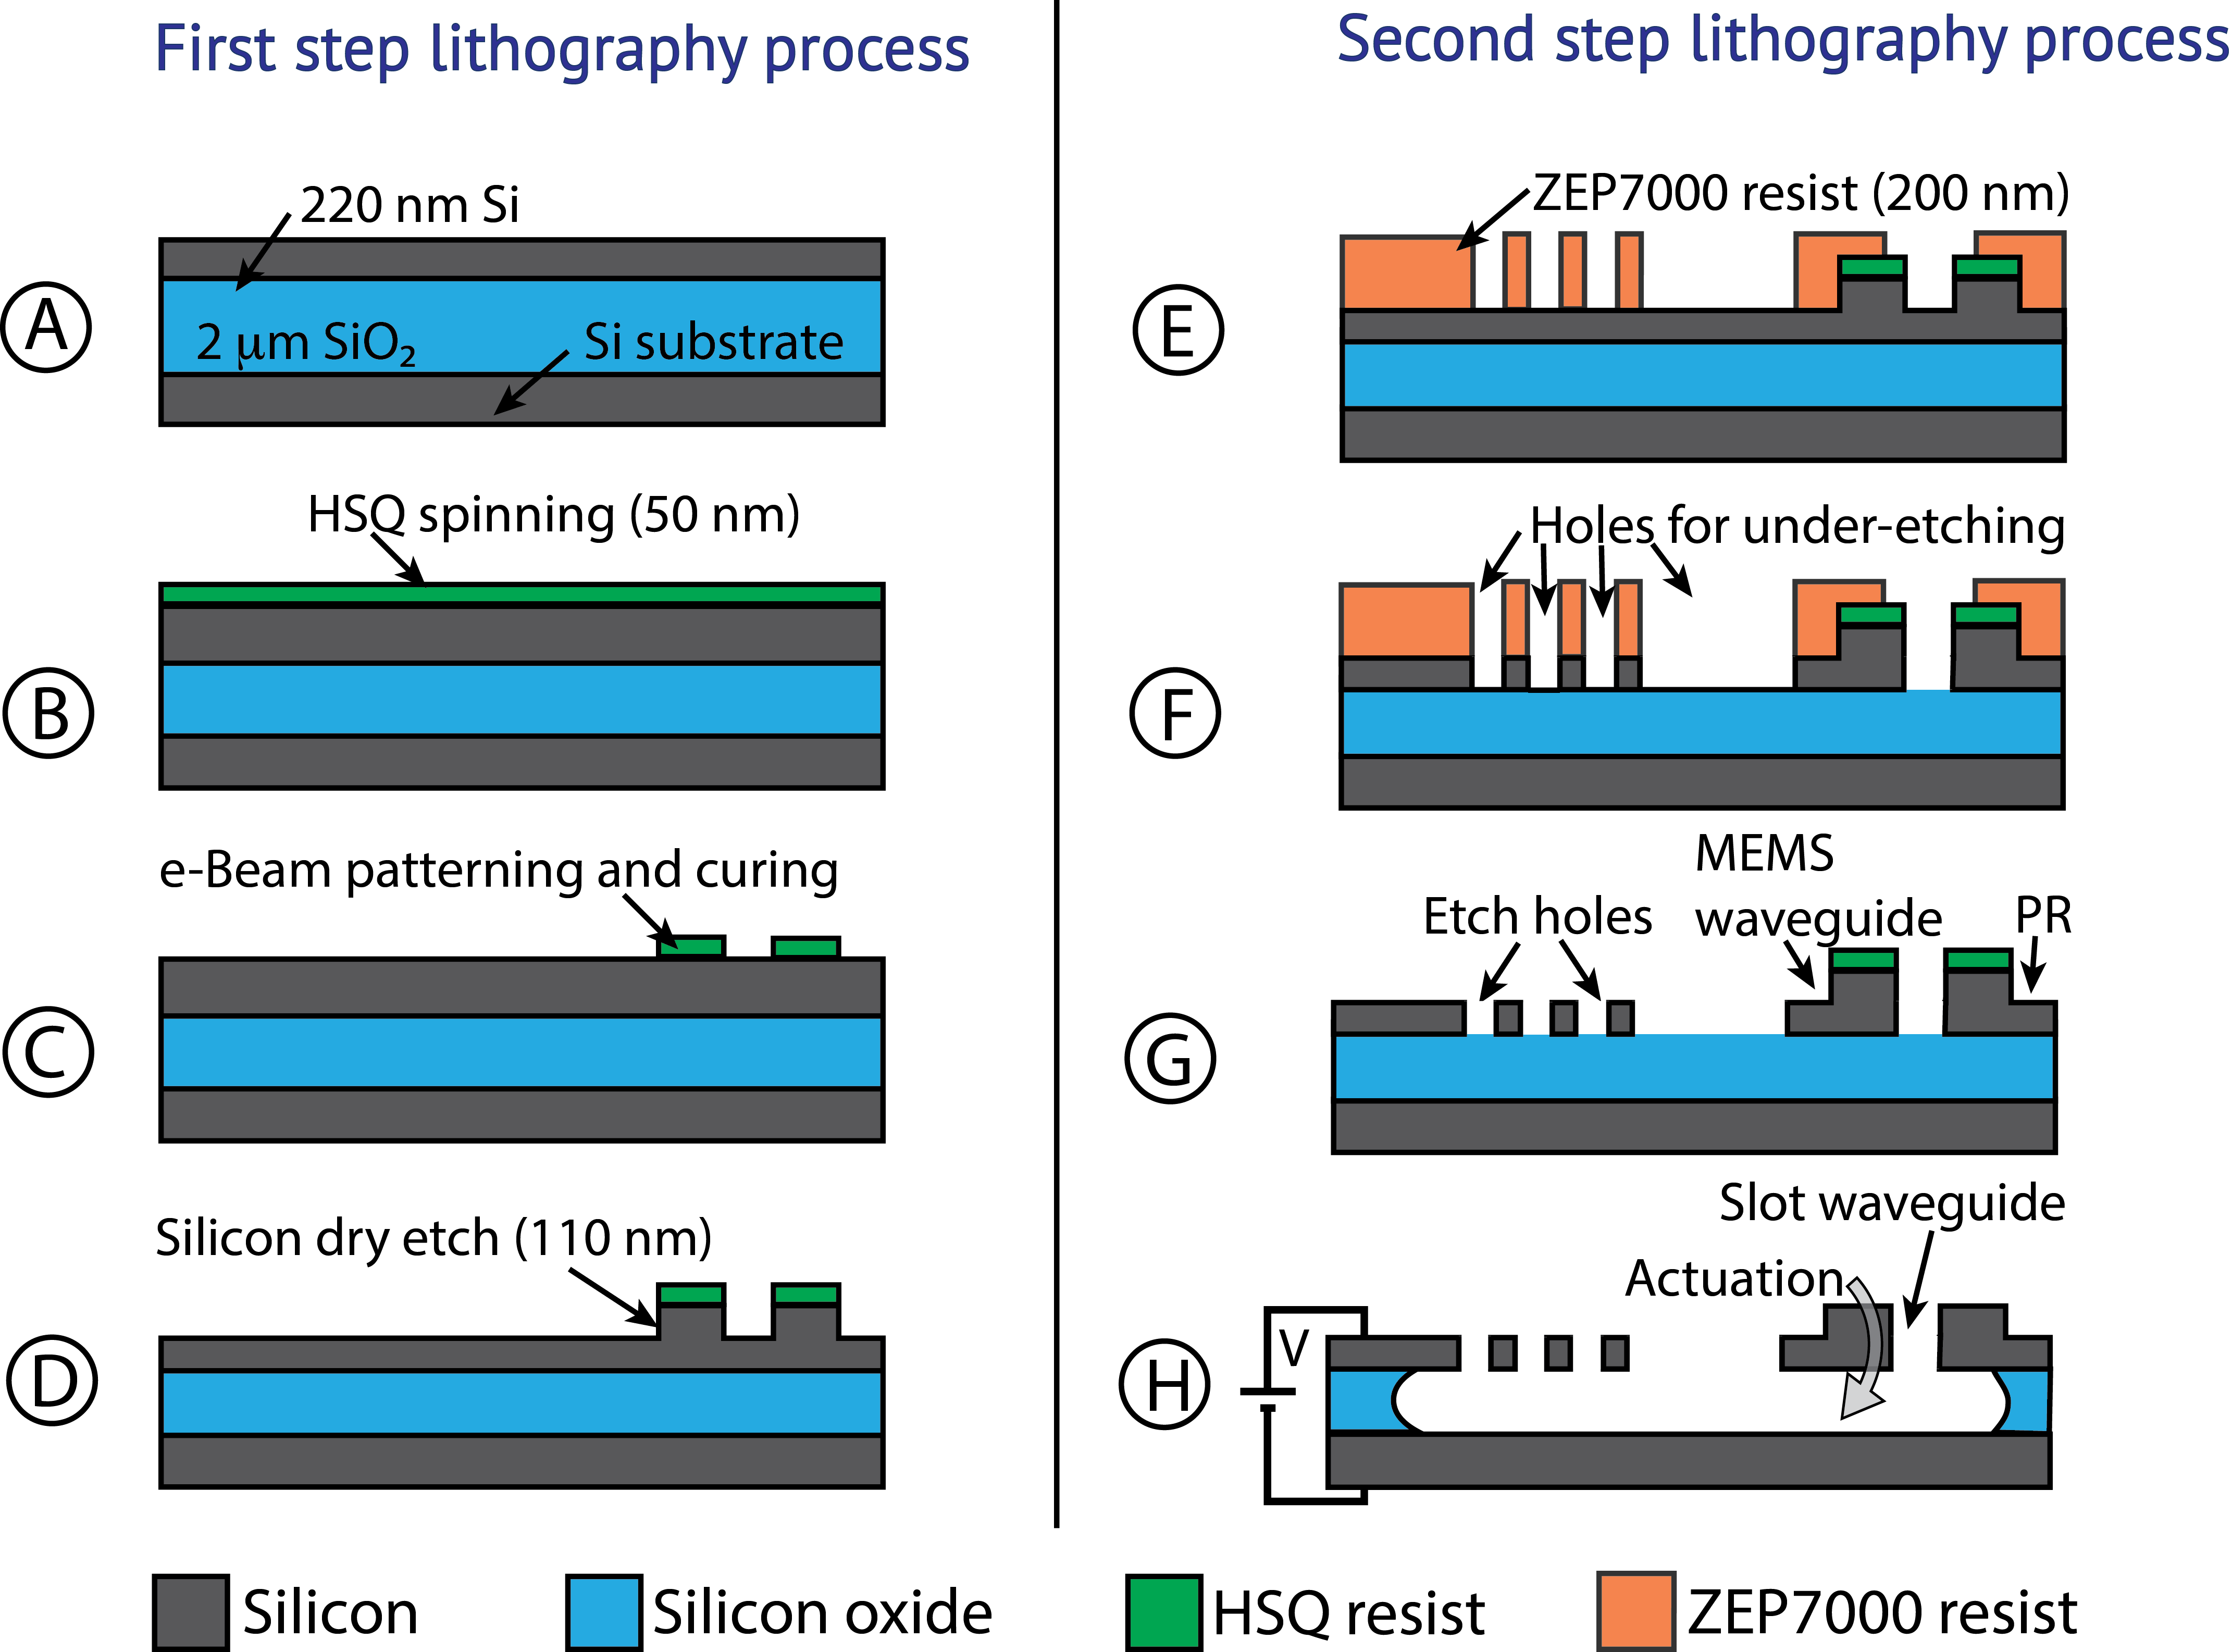
\includegraphics[width=1.0\textwidth]{5-fabrication}
	\caption{Cross-sectional schematic of the fabrication process}
	\label{fig:5_fabrication}
\end{figure}

% The fabrication process starts with a clean SOI chip with a \SI{220}{\nano \meter} crystalline silicon device layer and \SI{2}{\micro \meter} buried oxide (\ref{fig:4_fabrication} A). This is a standard substrate specification used by the Epixfab silicon photonics foundries. Electron beam patterning of a \SI{50}{\nano \meter} layer of a high-resolution negative electron beam resist (\gls{hsq}) defines the waveguide structures (\ref{fig:4_fabrication} B). The pattern is then transferred to the device layer by timed dry etch of silicon, resulting in ridge waveguide structures with \SI{110}{\nano \meter} height on a \SI{110}{\nano \meter} thick silicon slab ((\ref{fig:4_fabrication} C)). The patterned \gls{hsq} remains on the chip for the next lithography step.
%$\chem{H_2} + (1/2)\,\chem{O_2} = \chem{H_2O}$

\subsection{Piranha bath}			
The fabrication process starts with cleaning the \gls{soi} chip with \SI{220}{\nano \meter} crystalline silicon device layer and \SI{2}{\micro \meter} buried oxide, in the piranha solution (Fig. \ref{fig:5_fabrication} A). Piranha solution is a mixture of sulfuric acid ($\chem{H_2SO_4}$) and hydrogen peroxide ($\chem{H_2O_2}$), used to clean organic residues off substrates. Because the mixture is a strong oxidizing agent, it will remove most organic matter, and it will also hydroxylate most surfaces (add OH groups), making them highly hydrophilic (water-compatible) \cite{piranha_bath}. 
 
\subsection{HSQ resist spin}
A \gls{hsq} negative resist is spun on the \gls{soi} chip to create a thickness of \SI{50}{\nano \meter}. This is achieved by spinning the chip on a  rotating platform at 4000rpm for 30 seconds. The \gls{hsq} layer is hardened by baking the chip on a hot plate at $\chem{170^{\circ}}$ C for 5 minutes. To measure the thickness of sample a scratch is made on the chip and checked for depth variations using mechanical profilometer (KLA-Tencor). This is done to verify the profile depth of the mask.

\subsection{First e-beam exposure}
To develop the chip, selective portions of the chip are exposed using e-beam. E-beam exposure exceeds patterning capability of optical lithography and creates patterns in sub-microns scale. Before loading the chip into the chamber via the sample stage, pressure is adjusted with the external environment. Initially, one corner of the chip is scratched to align the chip and find particles on the chip to focus the beam correctly. Write-field alignment is a very central adjustment in the process of getting the best possible e-beam lithographic result. It is the adjustment of the electromagnetic/electrostatic deflections system inside the column to the high precision X-Y-Z stage. The stage is considered to be ``correct'' and the e-beam deflection system is aligned to it. To increase the dose in certain portions of the chip (CAD drawn using Raith 150 e-beam lithography software), the scanning speed is slowed down so that more electrons can strike the \gls{hsq} surface and expose it with a higher dose. The chip is developed using ma-D 525 (micro-resist) which dissolves non-hardened \gls{hsq}. The chip is then put in water to dissolve ma-D 525 and dried using nitrogen. Finally, the exposed \gls{hsq} in the chip is hardened more by putting it in an oven for 40 minutes at $\chem{400^{\circ}}$ C. The chip is cleaned and covered with ceramic glass which avoids deposition of dust cloud. After this step the chip resembles the diagram in Fig. \ref{fig:5_fabrication} C. Again mechanical profilometer is used to verify the thickness of \gls{hsq}.    

\subsection{First dry etch step}
The device pattern is finally transferred to the device layer by a timed ($\chem{HBr}$) dry etching of silicon ($\approx$ 35 seconds), resulting in ridge waveguides with \SI{110}{\nano \meter} height on a \SI{110}{\nano \meter} thick silicon slab (Fig. \ref{fig:5_fabrication} D). The patterned \gls{hsq} remains on the chip for the next lithography step. Finally, optical profiling is performed to find out the depth of the silicon etch. This process marks the end of the first step lithography process.

\subsection{ZEP7000 spin}
A ZEP7000 resist (positive) is applied on the chip by using an eppendorf pipette. To achieve a ZEP profile of \SI{200}{\nano \meter} thickness the platform is rotated at 3000 rpm for 45 seconds. The sample is baked at $\chem{170^{\circ}}$ C for 3 minutes to make the ZEP layer harder. After this, a scratch is then made on the sample and the profile depth is measured using a mechanical profilometer (KLA-Tencor).

\subsection{Second e-beam exposure}
Before the second e-beam exposure, local axis alignment is needed because it is a two-step fabrication. Some unique and easily recognizable feature like plus symbol is selected as a mark, patterned in the first exposure. The contamination dots from the focusing is a good example. Write-field alignment is performed in all the cells manually for dimensional precision \cite{write_field}. Since ZEP is a positive resist, the exposed portions are developed using p-Xylene solvent and MIBK. After developing the chip, the cross-section looks like Fig. \ref{fig:5_fabrication} E.

\subsection{Second dry etch step}
The double step device pattern is obtained in the device layer when all the remaining silicon is etched. This is done via another dry etch step similar to the previous one ($\approx$ 35 seconds). The goal of this dry etch process is to etch through the remaining silicon via the holes created using ZEP resist. The ZEP polymer is cleaned via resist stripping using oxygen plasma. After this process the device cross-section looks like Fig. \ref{fig:5_fabrication} F. 

\subsection{Wet etching and critical point drying}
The final step in the fabrication process consists of removing the \gls{hsq} and the underlying $\chem{SiO_2}$. This is done via wet etching using HF for 200 seconds. The HF is diluted using cold water and then the chip is transferred to isopropanol ($\chem{CH_3CHOHCH_3}$). Drying \gls{mems} in air or under vacuum can drastically alter their structures or even destroy them completely. A gentle method for such purposes is critical point drying. The surface tension of the water and isopropanol in a micro device is at the point at which a change from liquid to gaseous state can destroy the device through capillary forces. By increasing the pressure and temperature of the substrate it is possible to dry without crossing a phase boundary. This is possible because once the critical point has been passed, the density of liquid and gas are the same. $\chem{CO_2}$ is a good transitional fluid for which the critical point temperature and pressure are relatively low and hence the \gls{mems} structures are not destroyed. After the critical point drying the device is developed with the structure as in Fig. \ref{fig:5_fabrication} H. 

\section{Final product}

Show SEM image

\end{document}
